\section{Skalowalność i wysoka dostępność}
Rozdział rozpocznę od wyjaśnienia kilku terminów i teorii, które będą przydatne podczas dalszego rozważania problemów wydajności i wysokiej dostępności MySQL.


\subsection{Terminologia}
\subsubsection{Skalowalność a wydajność}
Rozpoczynając ten rozdział najważniejszym zadaniem jest wyjaśnienie różnicy pomiędzy skalowalnością, a wydajnością. Termin\textit{wydajność} w informatyce dotyczy ilości danych przetwarzanych w czasie. W przypadku baz danych termin ten może dotyczyć na przykład: ilości jednoczesnych połączeń do bazy danych, liczbie zapytań wykonywanych na sekundę lub rozmiar odczytywanych danych. Natomiast \textit{skalowalność} oznacza możliwość aplikacji do zwiększenia wydajności. Skalowalny system to taki, w którym w najgorszym przypadku wzrost kosztów wynikający ze zwiększenia zasobów jest liniowy do wzrostu wydajności, jakie te zasoby zapewniają. Innymi słowy możliwy jest system, który jest bardzo wydajny, ale bardzo słabo skalowany. Możliwy jest także system niewydajny, który jest bardzo dobrze skalowany, dlatego istotnym jest, żeby nie mylić tych pojęć.


\subsubsection{Teoria CAP}
Autorem teorii CAP jest Eric Brewer, który przypisał bazą danych trzy własności:
\begin{itemize}
	\item Spójność (eng. \textit{Consistency}), oznaczająca, że odpytując dowolny działający węzeł, zawsze otrzymamy takie same dane.
	\item Dostępność (eng. \textit{Availability}), określająca możliwość zapisywania i odczytywania danych nawet w przypadku awarii dowolnego węzła.
	\item Odporność na podział (eng. \textit{Partition Tolerance}), pozwalająca na rozproszenie niewrażliwe na awarię.
\end{itemize}
Istotą teorii CAP jest stwierdzenie, że baza danych może spełniać co najwyżej dwie spośród trzech wymienionych wyżej własności. Konkluzją z powyższego stwierdzenia jest fakt nieistnienia idealnej bazy danych i każda z nich jest pewnym kompromisem, kładącym nacisk na pewne własności, kosztem innych.

\subsubsection{Skalowanie wertykalne i horyzontalne}
Skalowaniem wertykalnym nazywamy zwiększenie wydajności w ramach jednej monolitycznej maszyny. Takie rozwiązanie jest skuteczne tylko do pewnego momentu. Wraz z wzrostem wydajności, takie rozwiązanie będzie się wiązało z dużym wzrostem kosztów, nawet przy małym wzroście możliwości serwera. Ostatecznie osiągniemy limit możliwości jednej maszyny i zwiększenie wydajności nie będzie dalej możliwe. Dodatkowo sam serwer MySQL ma problemy z wykorzystywaniem większej ilości procesorów i dysków twardych. Kolejnym utrudnieniem jest fakt, że MySQL nie potrafi obsłużyć pojedyńczego zapytania na kilku procesorach, co jest sporym utrudnieniem przy zapytaniach, które mocno obciążają procesor maszyny. Z powodu wyżej wymienionych ograniczeń skalowania pionowego, nie jest ono zalecane, jeżeli aplikacja ma zapewnić wysoką skalowalność.

W przeciwieństwie do skalowania wertykalnego, w modelu skalowalności horyzontalnej zwiększenie wydajności odbywa się przez dodanie kolejnych serwerów, przy zachowaniu wydajności pojedynczych serwerów. W kolejnych podrozdziałach zostaną przedstawione różne sposoby realizacji modelu skalowania horyzontalnego. Takie rozwiązanie jest zdecydowanie tańsze i teoretycznie nie posiada limitu wydajności. Niestety wraz ze wzrostem liczby serwerów, rosną też problemy z zachowaniem spójności pomiędzy poszczególnymi węzłami.


\subsection{Architektura master-slave}
Najpopularniejszym sposobem skalowania horyzontalnego jest realizacja architektury \textit{master-slave}. Rozwiązanie polega na podziale serwerów bazodanowych na jeden serwer nadrzędny (\textit{master}) oraz wiele serwerów podrzędnych (\textit{slave}). Replikacja danych opiera się na następującej zasadzie. Serwer nadrzędny obsługuje wszystkie operacje, które modyfikują dane (zapis, odczyt, aktualizacja), równocześnie rejestrując każdą operację, która wykonał. Następnie każdy z serwerów podrzędnych odczytuje rejestr operacji i aktualizuje swój stan. Efektem tej pracy jest wiele instancji bazy danych zawierających identyczne dane. Co kiekawe możliwe jest takie skonfigurowanie mechanizmu replikacji, żeby replikowane były dane z tylko niektórych schematów, lub nawet pojedynczych tabel.
Taki podział ma wiele zalet. Przede wszystkim wyraźnie zwiększone zostaje wydajość operacji odczytu, ponieważ mogą być realizowane równolegle przez wiele instacji serwera MySQL. Dodatkowo redundancja danych na wielu instancjach sprawia, że system staje się bardziej odporny na utratę danych spowodowaną awarią sprzętową. W przypadku awarii na którymkolwiek z serwerów, dane na innych instancjach umożliwią przywrócenie stanu sprzed awarii. Dodatkowo zmniejsza się zapotrzebowanie na tworzenie kopi zapasowych danych, co jest szcególnie przydatne przy dużych rozmiarach danych, ponieważ operacje tworzenia kopi zapasowych mogą być znaczącym obciążeniem dla serwera. Co więcej, operację \textit{backupu} danych można wykonać na serwerze \textit{slave}, co dodatkowo odciąża serwer główny. Replikacja danych w trybie \textit{master-slave} może odbywać się w jednym z następujących trybów:
\begin{itemize}
 	\item \textbf{SBR} (statement-based replication) - Najprostsza z metod. Zapisywane są tylko zapytania modyfikujące dane. SBR jest pierwszym typem replikacji stosowanym w MySQL. Tryb ten może jednak prowadzić do braku spójności danych na różnych serwerach \textit{slave}. Wyobraźmy sobie zapytanie, które zawiera funckję RAND() lub funkcje odwołujące się do aktualnego czasu. Takie zapytania wykonane na różnych serwerach mogą zmodyfikować w taki sposób, że będą one niespójne.
	\item \textbf{RBR} (row-based replication) - logowane są wyniki zapytań modyfikujących dane, czyli informacja o tym, który rekord i w jaki sposób został zmodyfikowany. Jest to domyślny typ replikacji w MYSQL 8. W porównaniu do metody SBR jest niestety wolniejsza i dodatkowo ziększa się ilość przesyłanych danych pomiędzy serwerem master i slave.
	\item \textbf{MFL} - połączenie dwóch powyższych metod. W tym trybie domyślnie używana jest metoda SBR, ale w niektórych sytuacjach wykorzystywana jest metoda RBR.
\end{itemize}

Rozwiązanie polegające na replikacji danych do serwerów podległych idealnie sprawdzi się w aplikacjach, które przechowują ograniczoną wielkość danych, oraz zdecydowana większość operacji, to operacje odczytu. Taka realizacja skalowania poziomego może nie sprawdzić się w systemach przechowujących ogromne ilości danych, ponieważ wymaga przechowywania wszystkich danych w każdym z węzłów, co może skutkować bardzo wysokimi kosztami utrzymania serwerów, a nawet być niemożliwe, jeżeli rozmiar danych przekracza możliwości pojedynczego węzła. Kolejmym przypadkiem, którego nie rozwiązuje mechanizm replikacji jest system, w którym większość operacji to operacje modyfikujące dane. W takim scenariuszu serwer nadrzędny stanie się wąskim gardłem, a dodatkowo dużą część obciążenia serwerów będzie stanowiła replikacja pomiędzy serwerem nadrzędnym i serwerami podrzędnymi, co dodatkowo zmniejszy wydajność operacji zapisów na serwerze nadrzędnym, który część zasobów będzie przeznaczał na przygotowanie plików replikacji. Reasumując skalowanie horyzontalne za pomocą mechanizmu replikacji \textit{master-slave} idealnie sprawdzi się , gdy zdecydowaną większością operacji, są operacje odczytu, a rozmiar danych jest ograniczony.

Skalowanie z zastosowaniem replikacji \textit{master-slave} jest często stosowane razem z \textit{load balancerem} (przykładowo ProxySQL), który odpowiada za balansowanie obciążenia operacji odczytu pomiędzy serwerami podrzędnymi oraz zapewnia rzeźroczystość dostępu do danych z punktu widzenia aplikacji, która ma wrażenie komunikowania się z tylko jednym serwerem. Przykład takiej architektura przedstawiono na poniższym diagramie.

\begin{figure}[!h]
	\caption{Przykładowa architektura master-slave z load balancerem}
	\centering
	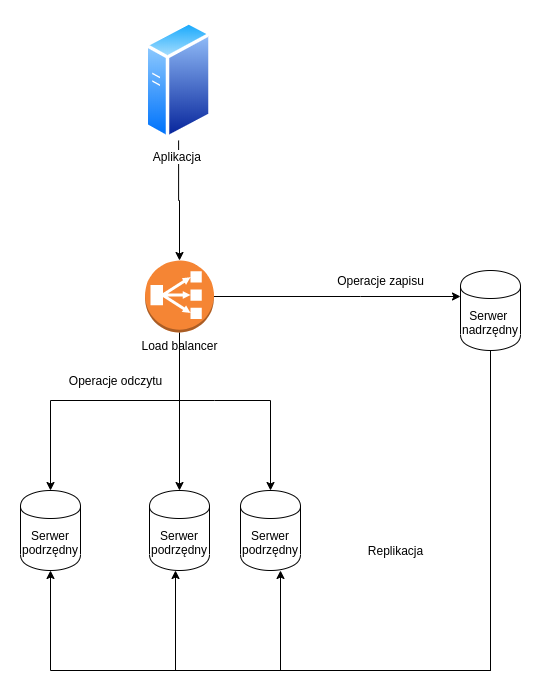
\includegraphics[scale = 0.35]{architektura-z-load-balancerem.png}
	\label{fig:label}
\end{figure}

\subsection{Architektura multi master}


\subsection{Partycjonowanie funkcjonalne}

Funkcje aplikacji można podzielić na pewne podgrupy, które nie łączą się z pozostałymi, na poziomie zapytań SQL. Przykładowo serwis społecznościowy \textit{Facebook} umożliwia odczytywania postów innych użytkoników oraz dokonywanie zakupów w sekcji \textit{Marketplace}. Jeżeli użytkownik przegląda aktualne oferty w dziale \textit{Marketplace}, to zapytania kierowane o bazę danych, będą odpytywać jedynie kilka tabel związanych z zakupami. Jeżeli w tym samym czasie inny użytkownik przegląda posty użytkowników, zapytania nie będą dotyczyć table związanych z zakupami. Oczywiście przykład, który przedstawiłem powyżej, może i z pewnością jest rozwiązany za pomocą podziału na osobne serwisy jeszcze na poziomie aplikacji, ale zakładając, że nasza aplikacja nie została podzielona na osobne serwisy i łączy się z jedną bazą danych. W takiej sytuacji obciążenie serwera MySQL jest sumą obciążeń związanych z postami i zakupami. W takim przypadku skutecznym rozwiązaniem jest podział danych pojedynczej aplikacji na zestaw tabel, które nigdy nie są ze sobą łączone. Oczywiście takiego partycjonowania danych nie można przeprowadzać w nieskończoność, ponieważ nie istnieje skończony zbiór tabel, które możemy w taki sposób podzielić. Dodatkowo w ramach każdej z grup jesteśmy ograniczeni możliwościami skalowania pionowego bazy danych. Wadą jest też zwiększona złożoność samej aplikacji, która musi obsłużyć kilka źródeł danych. 

\begin{center}
	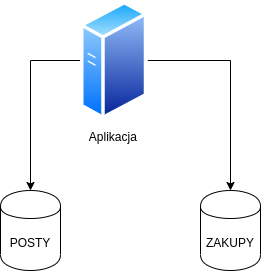
\includegraphics[scale = 0.7]{partycjonowanie-funkcjonalne.png} 
\end{center}


\subsection{Data-sharding}

\textit{Data-sharding} wykorzystuje fakt, że rekordy w ramach pojedynczej tabeli są niezależne od siebie. Jako przykład przeanalizujmy tabelę \textit{Comments} z naszej testowej bazy.
Wiersze w tabeli \textit{Comments} są logicznie powiązane z wierszami w tabeli \textit{Posts}, ale pomiędzy poszczególnymi wierszami w tabeli \textit{Comments} należącymi do innych postów, nie ma relacji. W naszej testowej bazie danych przechowujemy 25 milionów komentarzy. Z obsługą takiej ilości danych, baza danych nie powinna mieć problemów. Niestety z czasem tabela zawierająca komentarze może rozrosnąć się do rozmiarów, których obsłużenie w pojedynczej bazie danych może być problematyczne. Rozwiązaniem tego problemu może być podział pojedynczej tabeli na kilka baz danych. Możemy na przykład posty wraz z komentarzami o parzystym \textit{PostId} przechowywać w bazie danych A, a nieparzyste w bazie danych B. Dzięki temu, dwukrotnie zmniejszyliśmy liczbę zapytań do pojedynczej bazy danych, ilość wymaganego miejsca do przechowania postów i komentarzy, rozmiary buforów i indeksów. Wadą takiego rozwiązania jest konieczność obsługi sterowania zapytań do konkretnej bazy na poziomie aplikacji oraz wzrost złożoności logiki aplikacji i systemu bazy danych. Przykładowo chcąc pobrać najnowsze dziesięć postów, musimy wykonać dwa osobne zapytania, pobrać część redundatnych danych i na poziomie aplikacji dokonać wyboru dziesięciu najnowszych postów.
Głownymi przesłankami skłaniającymi do zastosowania tego sposobu skalowalności jest konieczność przechowywania danych w rozmiarach przekraczających możliwości jednego serwera lub skalowanie operacji zapisów, którego nie da się dokonać w ramach replikacji z jednym serwerem nadrzędnym. Sharding danych bardzo dobrze sprawdza się przy jednoczesnym zastosowaniu partycjonowania funkcjonalnego. Przykład zastosowania \textit{data-sharding} wraz z partycjonowaniem funkcjonalnym przedstawiono na poniższym schemacie.
\begin{center}
	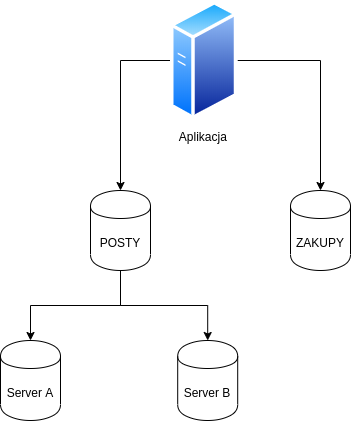
\includegraphics[scale = 0.7]{Partycjonowanie-funkcjonalne-sharding.png} 
\end{center}


\subsection{MySQL Cluster}